\documentclass[10pt,a4paper]{article}
\usepackage[utf8]{inputenc}
\usepackage[german]{babel}
\usepackage[T1]{fontenc}
\usepackage{amsmath}
\usepackage{amsfonts}
\usepackage{amssymb}
\usepackage{graphicx}
\usepackage{lmodern}
\usepackage{bm}
\usepackage{tikz}

\author{Lars Schiller}
\begin{document}


\section{Predicting the next pose of the robot}
\subsection{Modeling of Soft Bending Actuator}

\begin{itemize}
	\item Einführung virtueller Längen, um größeren Bereich erreichen zu können, und dennoch die Annahme von \textsl{Constant curvature} nutzen zu können.
	\item Weil Sehr effektiv zu rechnen.
\end{itemize}

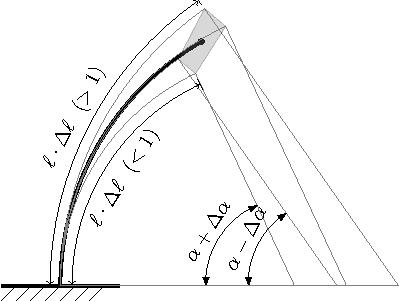
\includegraphics[scale=1]{pics/Virtual_length/virtual_length.pdf}



\subsection{Modeling of the robot}

	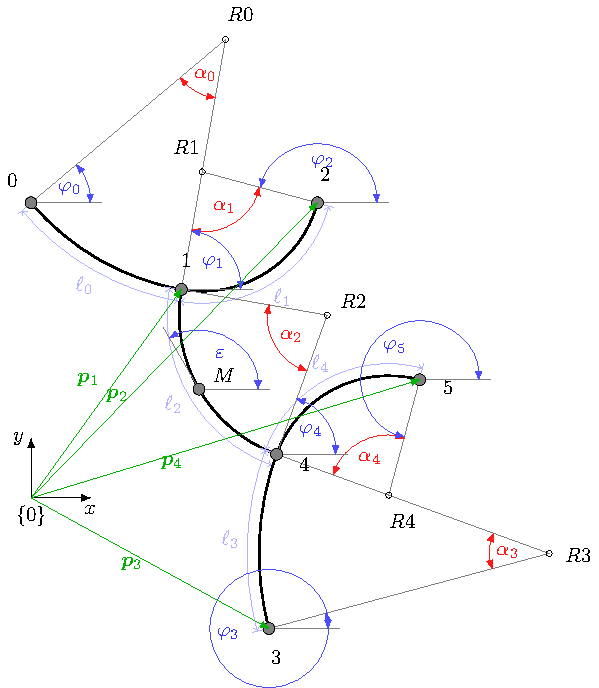
\includegraphics[scale=1]{pics/general_model/model_plain.pdf}

	\begin{itemize}
		\item Zustands- und Eingangsgrößen:
		$$
		\bm{x} = \left[~\bm{\alpha}~\bm{\ell}~\varepsilon~\right],~~~
		\bm{r} = \left[~\bm{\alpha}_{\textnormal{ref}}~\bm{f}~\right]
		$$
		
		\item Innere Spannung:
		$$
		\begin{array}{rcl}
		\sigma(\bm{x}_{k}) 
		&=&  w_\ell\big| \bm{\ell}_{k} - \bm{\ell}_n \big|_2 \\
		&&	+ w_\alpha\big| \bm{\alpha}_{k} - \bm{\alpha}_{\textnormal{ref},k} \big|_2 \\
		&&	+ w_\varphi \big| \textnormal{diag}(\bm{f}_k) ( \bm{\varphi}_{k} - \bm{\varphi}_{k-1}) \big|_2 \\
		\end{array}
		$$
		
		\item Minimale Spannung:
		$$
		\begin{array}{l}
		\displaystyle\min_{\bm{x}_k \in \mathcal{X}} ~ \sigma(\bm{x}_k) \\
		s.~t.~~~
		\big|\big|\textnormal{diag}(\bm{f}_k)(\bm{P}_{k} - \bm{P}_{k-1})\big|\big|_2 = 0
		\end{array}
		$$
		
		\item Folgepose:
		$$
		\bm{\rho}_k = [\bm{x}_k~\bm{P}_k~\bm{f}_k] = \textnormal{fun}_{\mathcal{P}}\left( \bm{r}_k, \bm{\rho}_{k-1} \right)
		$$
	\end{itemize}
	


\section{Path Planning with Search Tree}


\subsection{Different Gait Patterns for a curve}

\begin{itemize}
	\item Vom Kinematic Paper sind schon verschieden Laufmuster für Kurven bekannt, basierend auf dem Minimierungsproblem:
	
	\begin{equation}
		\displaystyle\min_{\bm{\alpha} \in \mathcal{A}} ~ \varepsilon(\bm{\alpha})
	\end{equation}
	
	wobei $\bm{\alpha}$ die Referenzwinkel von zwei Posen, also einem Zyklus enthält.

	\item Beispiele:

\end{itemize}

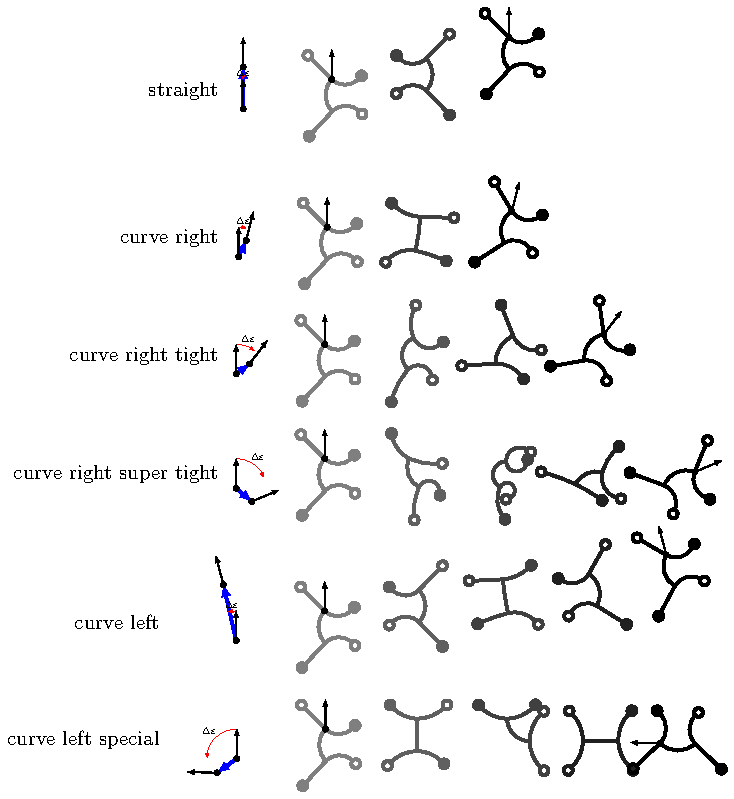
\includegraphics[width=.95\textwidth]{pics/trajectory_planner/elements.pdf}

\begin{itemize}
	\item Idee: Eine ausgewählte Anzahl an Posen, als Grundbausteine für einen beliebigen Gang.
	
	\item Diese dann wie Legosteine aufeinander setzen, um von A nach B zu gelangen.
\end{itemize}


\subsection{Search Tree}

\begin{itemize}
	\item Folgender Suchbaum wurde implementiert.
\end{itemize}

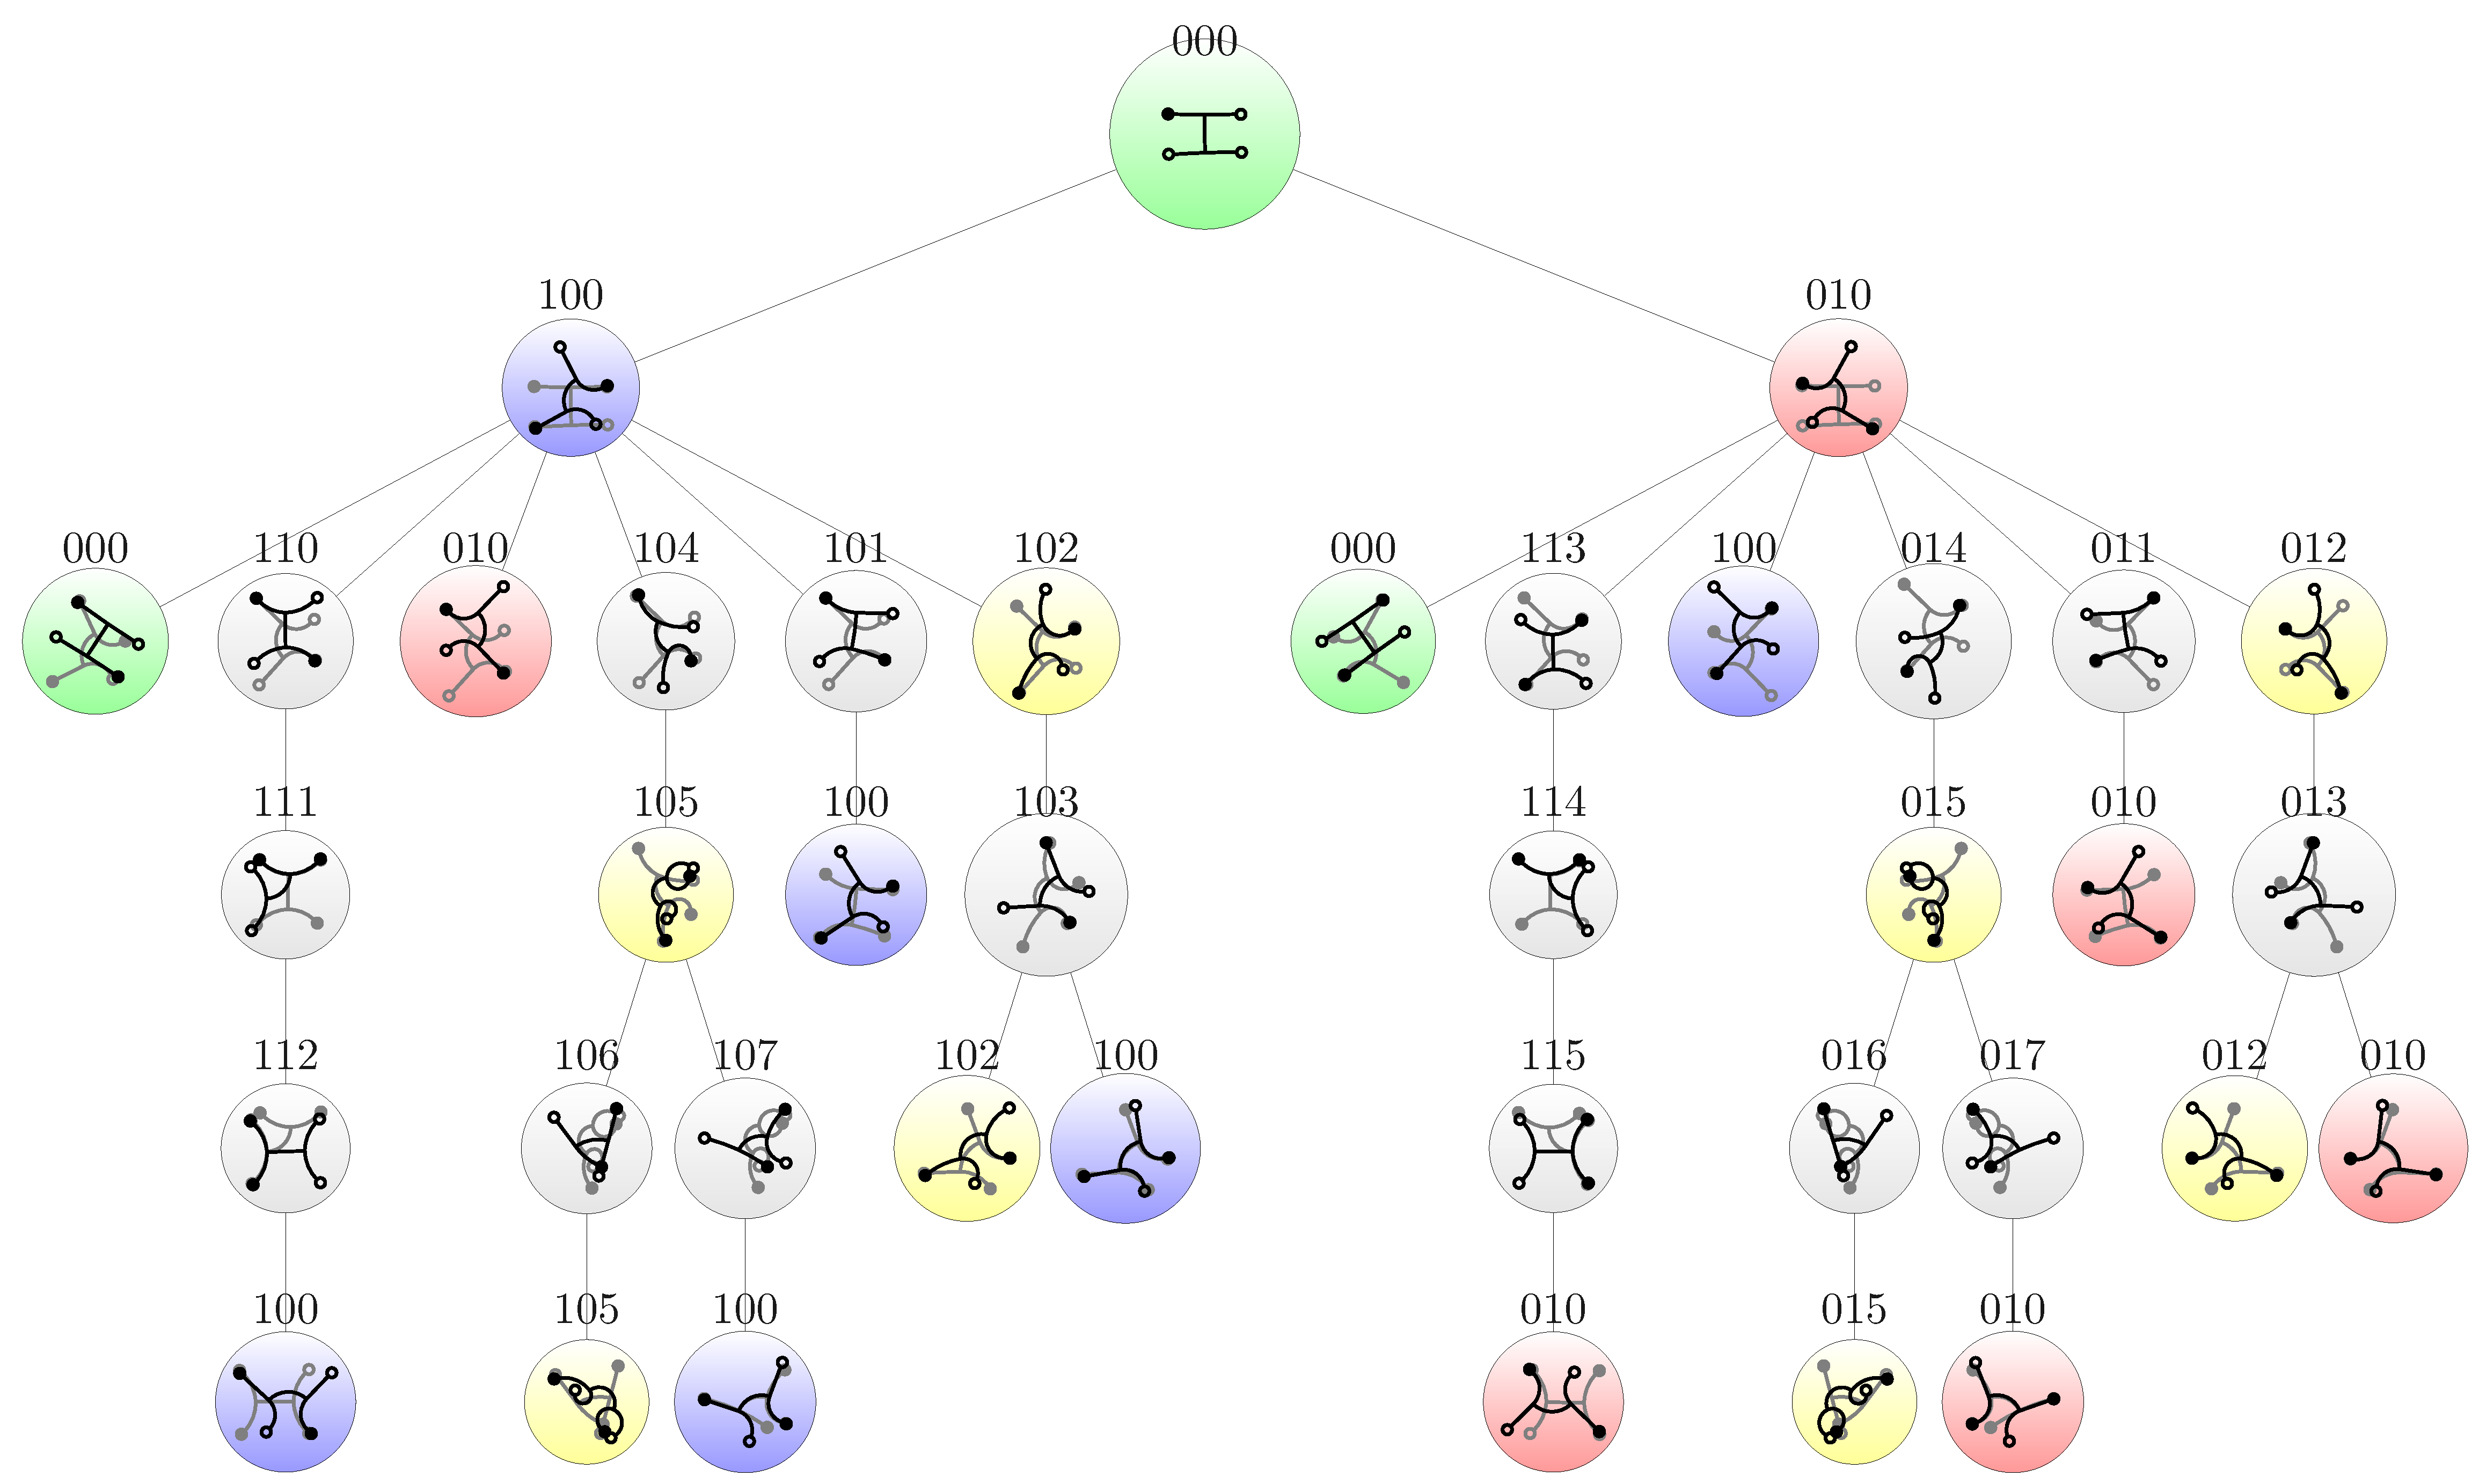
\includegraphics[width=.99\textwidth]{pics/trajectory_planner/tree.pdf}

\begin{tabular}{r|l}

\tikz\node[fill=green]{Green}; & Ruhe Pose \\
\tikz\node[fill=blue]{Blue}; & Rechte Adapter Pose\\
\tikz\node[fill=red]{Red}; & Linke Adapter Pose\\
\tikz\node[fill=yellow]{Yellow}; & Zwischen-Adapterpose für Kurven Looping\\
\tikz\node[fill=gray]{Gray}; & Zwischenpose \\

\end{tabular}

\begin{itemize}
	\item Dabei hat jede Kante des Baums eine Richtung und eine Gewichtung $w$.

	\item Die Gewichtung $w = ((\delta x, \delta y), \delta \varepsilon)$ gibt an, inwieweit das entsprechende Kind (Folgepose repräsentiert durch den Knoten, der mit der gewichteten Kante mit dem momentanen Knoten $k$ verbunden ist) den Roboter relativ zur momentanen Orientierung bewegt: $(\delta x, \delta y)$ und wie weit diese Pose ihn drehen wird: $\delta \varepsilon$.

	\item Für eine gegebene, momentane Pose $\bm{\rho}_k$ wird für alle Kandidaten $j \in [0,\cdots,J-1]$ ausgerechnet, wieweit der Abstand $d_j$ der potentiell neuen Pose $\bm{\rho}_j$ zum Ziel $\bar{\bm{x}}$ ist:

	\begin{equation}
	d(\bm{\rho}_k, w_j, \bar{\bm{x}}) = \bigg| \bar{\bm{x}} - \left(\bm{p}_{1,k} + \bm{R}(\varepsilon_k)\begin{bmatrix}
	\delta x \\ \delta y
\end{bmatrix}	 \right)\bigg|_2
	\end{equation}	
	
	\item Außerdem wird die Richtungsabweichung $\Delta \varepsilon_j$ aller potentiell neuen Pose $j$ berechnet:
	
	\begin{equation}
	\Delta \varepsilon (\bm{\rho}_k, w_j, \bar{\bm{x}}) = \measuredangle\left( \bar{\bm{x}} - \left(\bm{p}_{1,k} + \bm{R}(\varepsilon_0)\begin{bmatrix}
	\delta x \\ \delta y
\end{bmatrix} \right), \bm{R}(\varepsilon_k + \delta \varepsilon) \begin{bmatrix}
1 \\ 0
\end{bmatrix} \right)
	\end{equation}

	\item Die Folgepose $\bm{\rho}_{k+1}$ ergibt sich dann aus dem Minimum der mit $a=.5$ gewichteten Summe von Abstand und Orientierungsabweichung für alle Möglichkeiten $\bm{\rho}_{j}$:
	
	\begin{equation}
	\bm{\rho}_{k+1} = \min_j \left( a \frac{d_j}{d_{\textnormal{min}}}  + (a-1)\frac{\Delta \varepsilon_j}{\Delta \varepsilon_{\textnormal{max}}} \right)
	\end{equation}

	\item wobei $\Delta \varepsilon_{\textnormal{max}}$ die maximale Orientierungsabweichung aller Möglichkeiten ist; und $d_{\textnormal{min}}$ der minimale Abstand aller Möglichkeiten ist.

\end{itemize}


\subsection{Search Tree with weights}
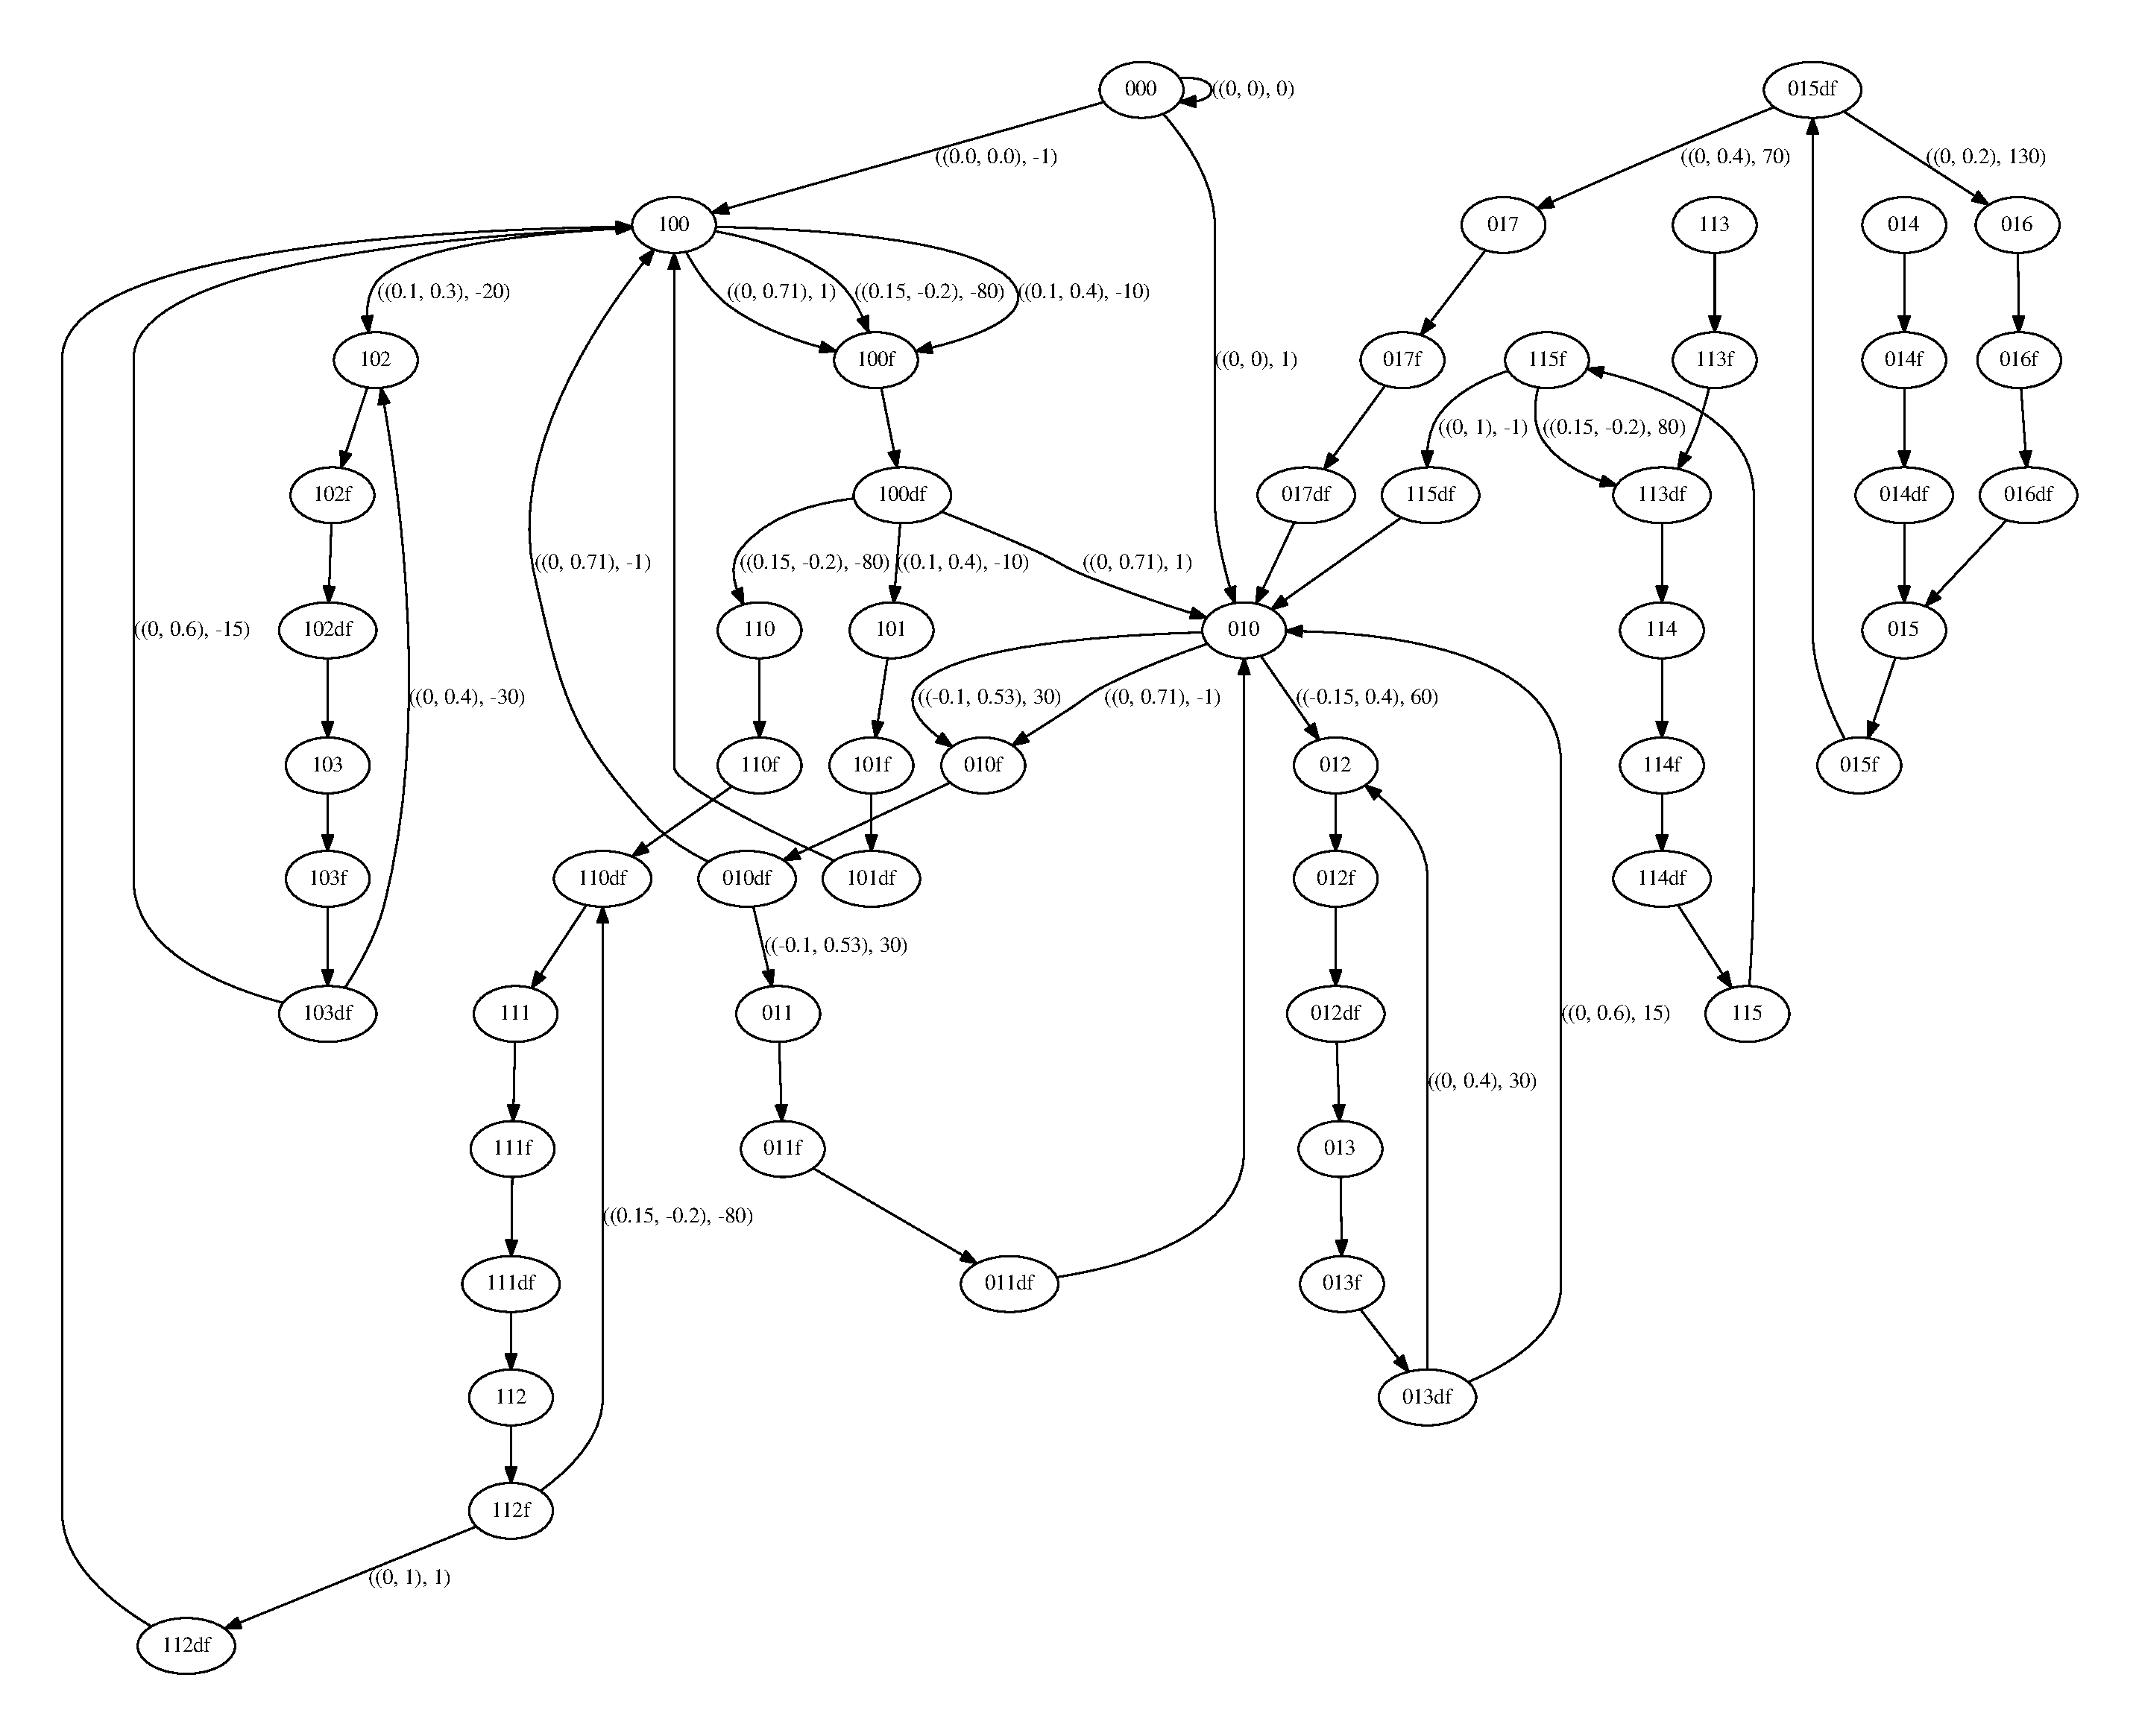
\includegraphics[width=.95\textwidth]{pics/trajectory_planner/tree_detail.pdf}

\subsection{Simulation Results Curve}

\begin{tabular}{ccc}
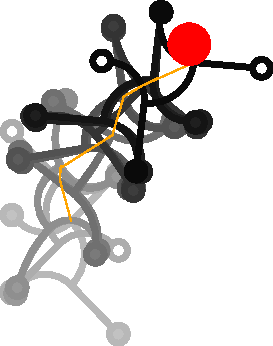
\includegraphics[width=.3\textwidth]{pics/pathplanner_without_noise/example_curve/gait.pdf}
&
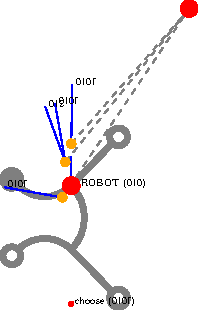
\includegraphics[width=.3\textwidth]{pics/pathplanner_without_noise/example_curve/dec_0.pdf}
&
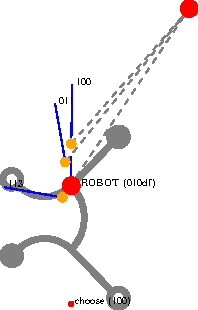
\includegraphics[width=.3\textwidth]{pics/pathplanner_without_noise/example_curve/dec_2.pdf}
\\
(a) & (b) & (c)
\\
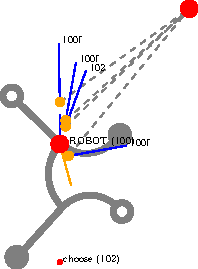
\includegraphics[width=.3\textwidth]{pics/pathplanner_without_noise/example_curve/dec_3.pdf}
&
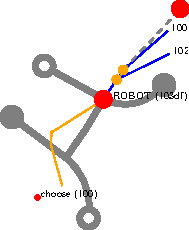
\includegraphics[width=.3\textwidth]{pics/pathplanner_without_noise/example_curve/dec_9.pdf}
&
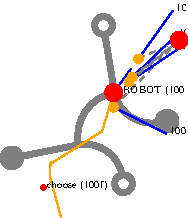
\includegraphics[width=.3\textwidth]{pics/pathplanner_without_noise/example_curve/dec_10.pdf}
\\
(d) & (e) & (f) 
\\
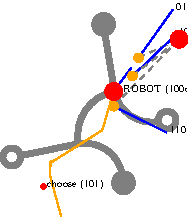
\includegraphics[width=.3\textwidth]{pics/pathplanner_without_noise/example_curve/dec_12.pdf}
&
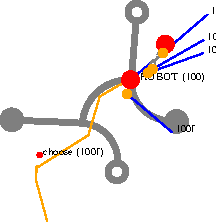
\includegraphics[width=.3\textwidth]{pics/pathplanner_without_noise/example_curve/dec_16.pdf}
&
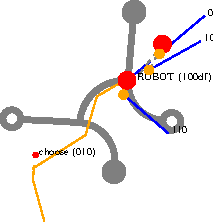
\includegraphics[width=.3\textwidth]{pics/pathplanner_without_noise/example_curve/dec_18.pdf}
\\
(g) & (h) & (i)\\
\end{tabular}

\subsection{Simulation Results Straight}
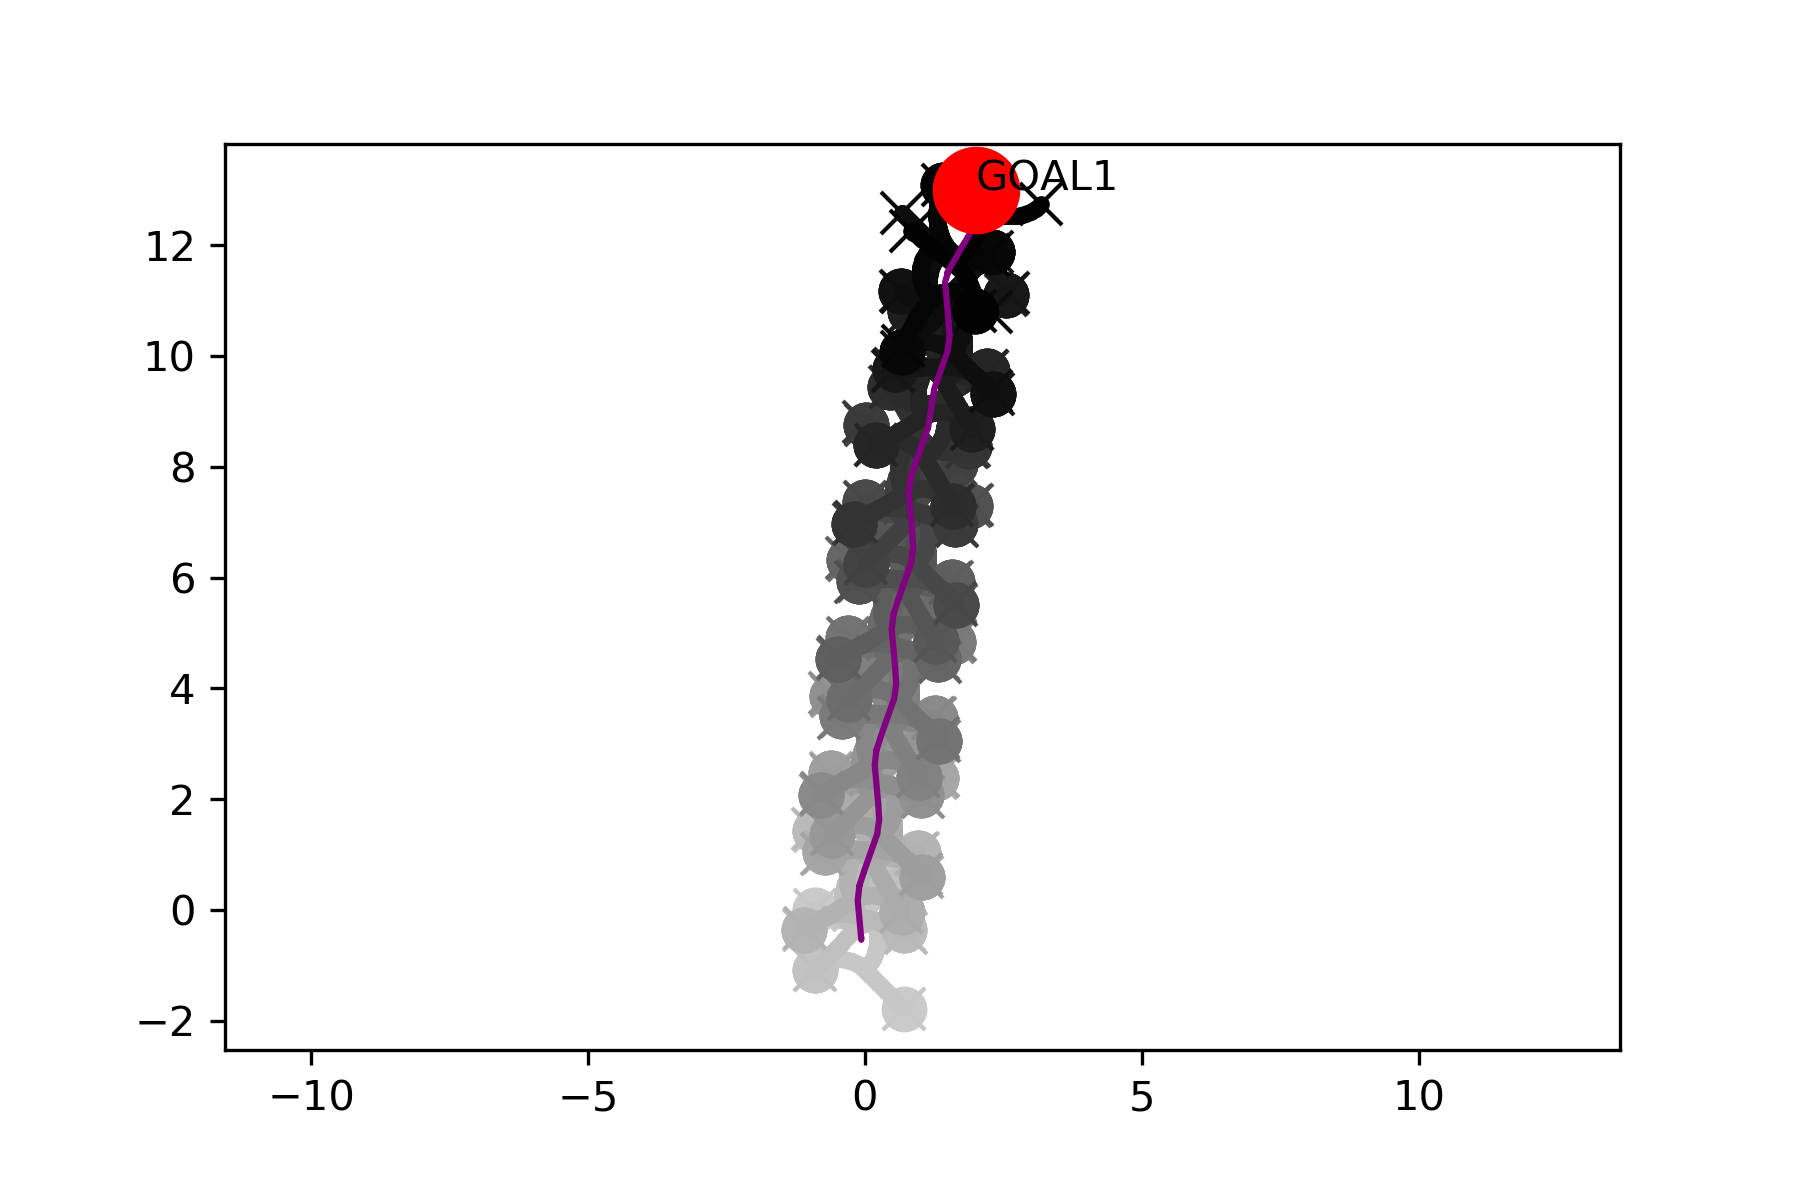
\includegraphics[width=.95\textwidth]{pics/pathplanner_without_noise/example_straight/gait.png}


\subsection{What happens if Process Noise occurs?}



\subsection{Conclusion}




\section{Path Planning with Analytic Model}

\subsection{Problem Statement}

\begin{itemize}

\item Angenommen die Konfiguration / Pose des Roboters $\bm{\rho} = [\bm{\alpha}, \bm{p}_1, \varepsilon]$ ist vollständig bekannt, wobei $\bm{\alpha}$ die Gelenkkoordinaten / Biegewinkel der einzelnen Glieder sind, $\bm{p}_1$ die Position des vorderen Torsoendes und $\varepsilon$ die Orientierung des Roboters.
Siehe Bild:

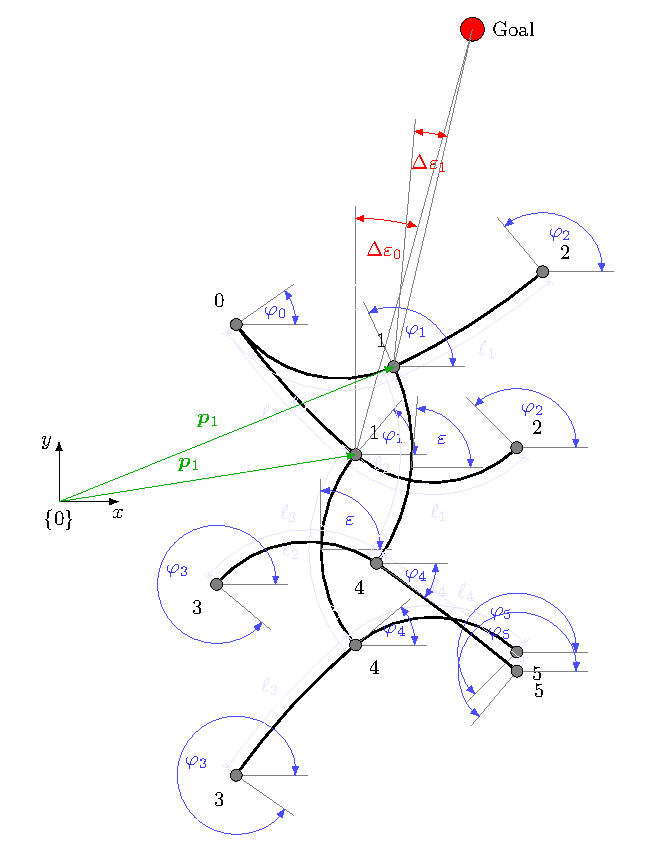
\includegraphics[width=8cm]{model.pdf}


\item Für die Pfadplanung, wäre eine Funktion hilfreich, die zu einer gegebenen Wunschdrehung $\Delta \varepsilon$, eine entsprechende Abfolge von Roboter-Konfigurationen / Posen ausgibt, sodass sich der Roboter entsprechend dreht.

\item So könnte zB die Richtung des Roboters so justiert werden, dass er sich auf ein gegebenes Ziel zu bewegt.


\item Für den geraden Gang ist eine analytische Funktion bekannt, die die Geschwindigkeit des Roboters einstellt. Geschwindigkeit im Sinne von Schrittweite, bzw. Vorschub pro Zyklus:

\begin{equation}
\bm{\alpha} = \begin{bmatrix}
45 - \frac{x_1}{2} \\
45 + \frac{x_1}{2} \\
x_1 \\
45 - \frac{x_1}{2}  \\
45 + \frac{x_1}{2} \\
\end{bmatrix}
\end{equation}

Die Schrittweite ist hier als $x_1$ beschrieben.

\end{itemize}




\subsection{Approach: Guess structure for a analytic model for walking curves}

\begin{itemize}

\item Src can be found: \texttt{analytic\_model.py}

\item Model:

$x_1$ beschreibt hier die Schrittweite

$x_2$ das Maß der Drehung.

\begin{equation}
\bm{\alpha} = \begin{bmatrix}
45 - \frac{x_1}{2} \\
45 + \frac{x_1}{2} \\
x_1 + x_2 \\
45 - \frac{x_1}{2}  \\
45 + \frac{x_1}{2} \\
\end{bmatrix}
\end{equation}

\item Method:

Simulate for different $x_1$ and $x_2$ (in der Abbildung unten ist $x_1$ = \texttt{gam} und $x_2$ = \texttt{x})

\item Results für 2 Zyklen:

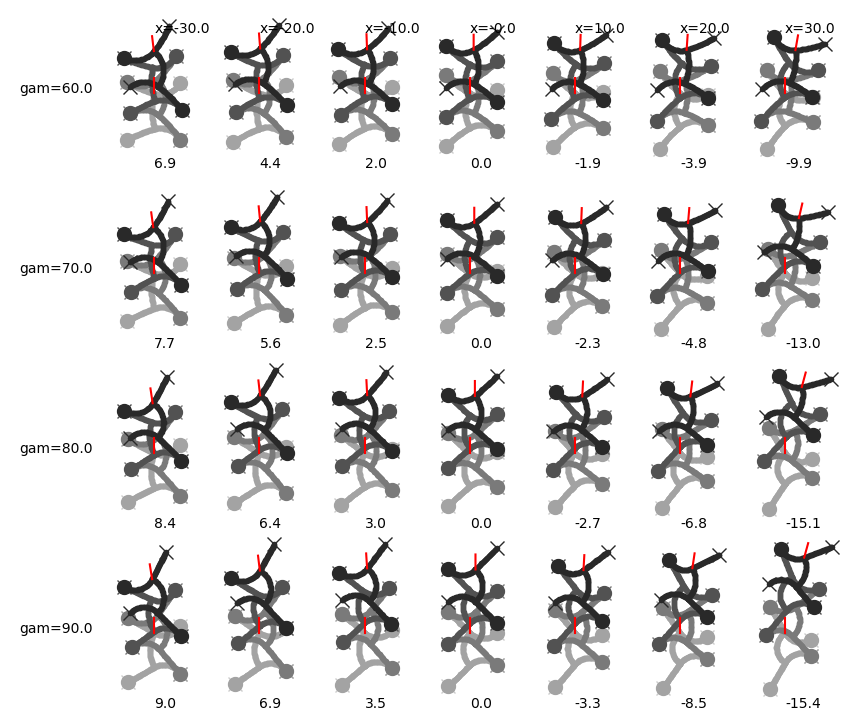
\includegraphics[width=12cm]{../pics/model_1/GeckoBotGait_2cyc.png}


\item Observations:

\begin{itemize}
	\item Es funktioniert. Der Roboter läuft eine Kurve.
	\item Kurve ist unsymmetrisch. Rechts klappt besser als links.
	\item Startpose ist besser für Rechtskurve geeignet.
	\item Noch nichts über die innere SPannung des Roboters herausgefunden
\end{itemize}



\end{itemize}


\subsection{Approach: Find a reasonable structure}

\begin{itemize}

\item Src can be found: \texttt{analytic\_model\_2.py}

\item Orientierung der Füße soll konstant bleiben:

\begin{equation}
\varphi_0 = \varepsilon + \frac{\alpha_2}{2} - \alpha_0
\end{equation}

Da im vorhergegangenem Versuch die asymmetrischen Aktuierung des Torsos schon zu guten Ergebnissen geführt hat, soll dieses Modell beibehalten werden. Allerdings in einer leicht variierten Form. $x_2$ ist nun ein relatives Maß für die Drehung:
\begin{equation}
\alpha_2 = x_1 + x_2|x_1|
\end{equation}


Es muss also $\alpha_0$ so gewählt werden, dass $\varphi_0$ möglichst unabhängig von $x_i$ wird.
Deshalb wird ein noch unbekannter Term $x_3$ hinzugefügt. Damit ergibt sich der Biegewinkel des Beines:

\begin{equation}
\alpha_0 = 45+ \frac{x_1}{2} + x_3.
\end{equation}

Für die Orientierung des Fußes bedeutet das:
\begin{eqnarray}
\varphi_0 &=& \varepsilon + \frac{x_1 + x_2|x_1|}{2} - \left( 45 + \frac{x_1}{2} + x_3 \right) \\
			&=& \varepsilon -45 + \frac{x_2|x_1|}{2} -x_3 \\
\end{eqnarray}

Es wird \textbf{angenommen}, dass die Orientierung des Roboters mit der Schrittweite linear wächst (i.e. Der Roboter dreht sich ein wenig zwischen seinen Extremposen):
\begin{equation}
\varepsilon = c_1 x_1 + \varepsilon_0
\end{equation}

Mit konstantem Orientierungswinkel $\varphi = \varphi_0$ ergibt sich somit:

\begin{eqnarray}
\varphi_0 &=& c_1 x_1 + \varepsilon_0 - 45 + \frac{x_2|x_1|}{2} -x_3 \\
x_3 &=&  c_1 x_1 + \frac{x_2|x_1|}{2} + c
\end{eqnarray}

Unter der \textbf{Annahme}, dass $\varphi_0 \approx \varepsilon_0 - 45$ ist, ergibt sich $c \approx 0$. Das meint, die Orientierung ändert sich nur minimal. entspricht also im Wesentlichen der Ausgangskonfiguration.
Weiterhin wird \textbf{angenommen}, dass für einen fixierter Fuß der Term $c_1x_1 \approx 0$ vernachlässigbar ist.
Somit ergibt sich für den Biegewinkel des fixierten vorderen linken Beins:

\begin{equation}
\alpha_{0,f} = 45-\frac{x_1}{2} + \frac{1}{2}x_2|x1|
\end{equation}

Wenn das Bein nicht fixiert ist, kann es beliebige Orientierung annehmen.
Hierfür wird \textbf{angenommen}, dass sich die Drehung des Körpers erst in der nicht fixierten Phase eines Beines in desses Orientierung auswirkt.
Deshalb, wird der Term $c_1x_1$ in dieser Phase aktiv.
Weiterhin wird \textbf{angenommen}, dass $c_1 = x_2$. Damit ergibt sich für einen nicht fixierten Fuß:

\begin{equation}
\alpha_{0,\bar{f}} = 45-\frac{x_1}{2} + x_2x1
\end{equation}


\item Das resultierende Modell sieht so aus:

\begin{equation}
\bm{\alpha} = \begin{bmatrix}
45 - \frac{x_1}{2}+ f_0\frac{1}{2}|x1|x_2  + \bar{f}_0x_1x_2  \\
45 + \frac{x_1}{2} + f_1\frac{1}{2}|x1|x_2+ \bar{f}_1x_1x_2  \\
x_1 + |x_1|x_2 \\
45 - \frac{x_1}{2}  + f_2\frac{1}{2}|x1|x_2 + \bar{f}_2x_1x_2\\
45 + \frac{x_1}{2}  + f_3\frac{1}{2}|x1|x_2+ \bar{f}_3x_1x_2 \\
\end{bmatrix}
\end{equation}

Wobei $f_i$ den Zustand des Fußes beschreibt:

\begin{equation}
f_i = \left[
\begin{matrix}
1 & if & \textnormal{foot fixed} \\ 
0 & else& \\
\end{matrix} \right.
\end{equation}
\begin{equation}
\bar{f}_i = \left[
\begin{matrix}
0 & if& \textnormal{foot fixed} \\ 
1 & else& \\
\end{matrix} \right.
\end{equation}

\item Results
\end{itemize}
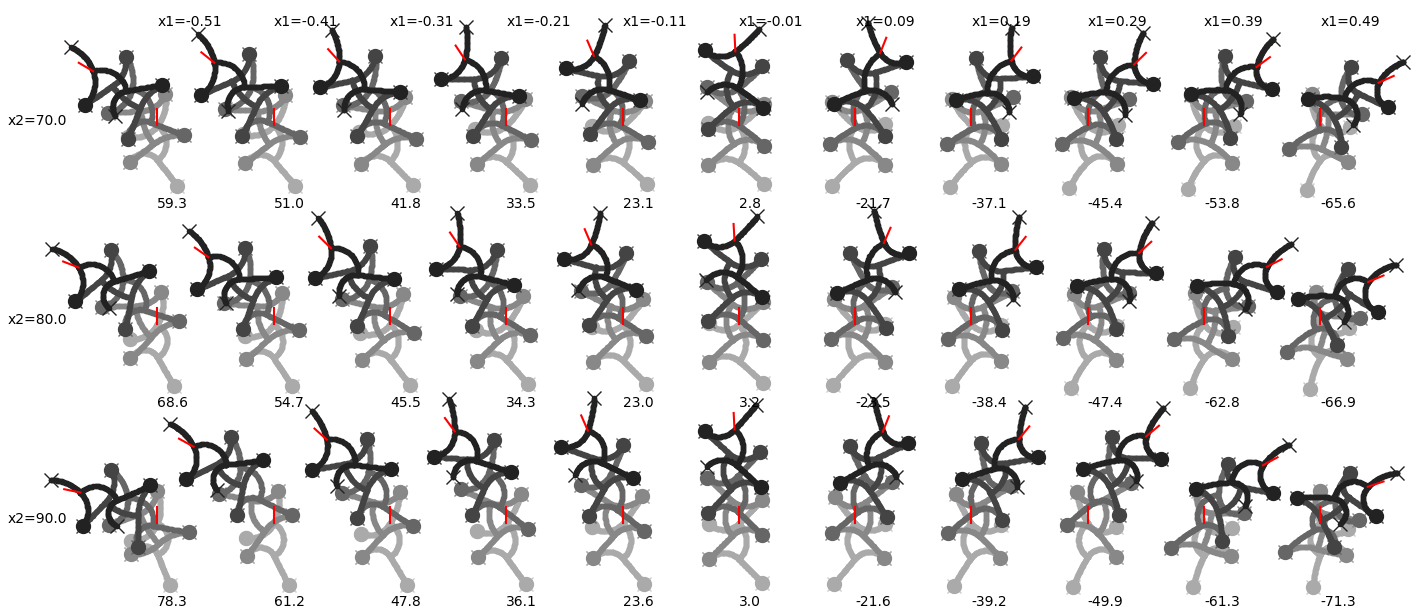
\includegraphics[width=.95\textwidth]{../pics/model_2/GeckoBotGait_2cyc.png}

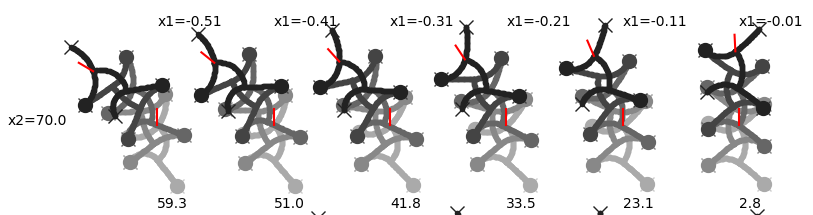
\includegraphics[width=.95\textwidth]{../pics/model_2/GeckoBotGait_2cyc_zoom.png}

Delta Epsilon: $\frac{\Delta \varepsilon}{cycle} (x_1, x_2) = f$

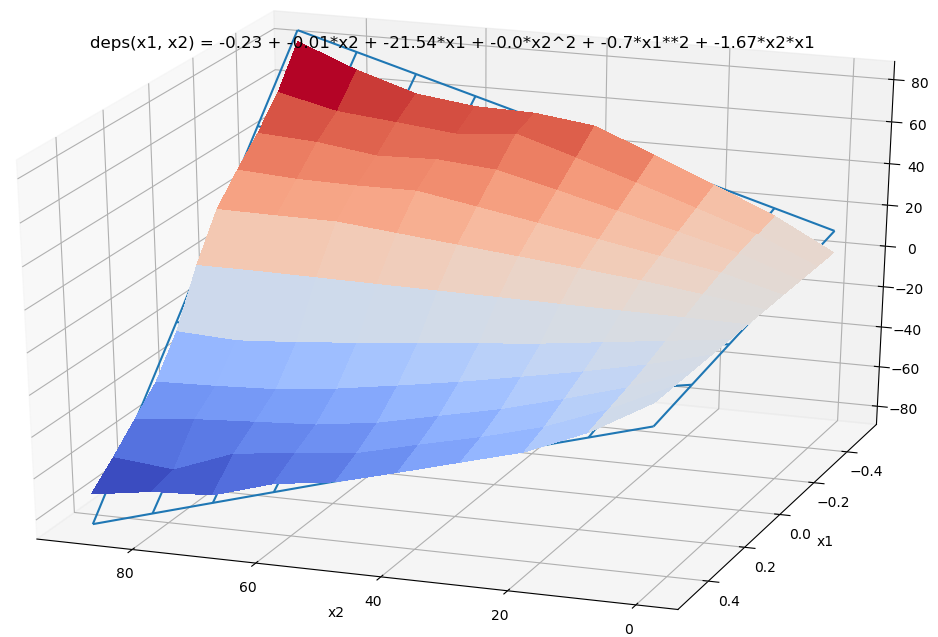
\includegraphics[width=.95\textwidth]{../pics/model_2/Delta_Epsilon_2cyc.png}



\subsection{Approach: Optimize Extra leg bending Angle for given extra torso bending}

\begin{itemize}

\item Src can be found: \texttt{analytic\_model\_3.py}


\item Nun soll untersucht werden, welche Extra Leg Bending Angle die ineere Spannung des Roboters minimiert.

\item Model:

\begin{equation}
\bm{\alpha} = \begin{bmatrix}
45 - \frac{x_1}{2} + \bar{f}_0x_3 + f_0x_4 \\
45 + \frac{x_1}{2} + \bar{f}_1x_3 + f_1x_4 \\
x_1|x_2| \\
45 - \frac{x_1}{2} + \bar{f}_2x_4 + f_3x_3 \\
45 + \frac{x_1}{2} + \bar{f}_3x_4 + f_4x_3 \\
\end{bmatrix}
\end{equation}


\item Annahme:

Die Extra Biegung $x_3$ für freie Beine und die Extra Biegung $x_4$ für fixierte Beine sind abhängig von der Extra Biegung $x_2$ für den Torso.

Hinter- und Vorderbeine sind nicht symmetrisch, aber kreuzweise symmetrisch:
Die Extrabiegung für ein \textbf{nicht fixiertes Vorderbein} entspricht der Extrabiegung eines \textbf{fixierten Hinterbeins} und anderesherum.


\item Methode:

Für gegebenes Extra Torso Bending $x_2$ und gegebenene Torso Biegung $x1$ minimiere die Innere Spannung über den Gang mit $n$ Zyklen aufsummiert:

\begin{tabular}{c c l}
Gegeben: 	& $x_1$ & Torsobiegung \\
			& $x_2$	& Extra Torsobiegung \\
Gesucht:	& $x_3$	& Extra Beinbiegung fixiert vorn \\
			& $x_4$	& Extra Beinbiegung fixiert hinten \\
\end{tabular}


\begin{equation}
cost(\bm{x}) = \sum gait(\bm{x}).stress
\end{equation}



\item Results:
\end{itemize}

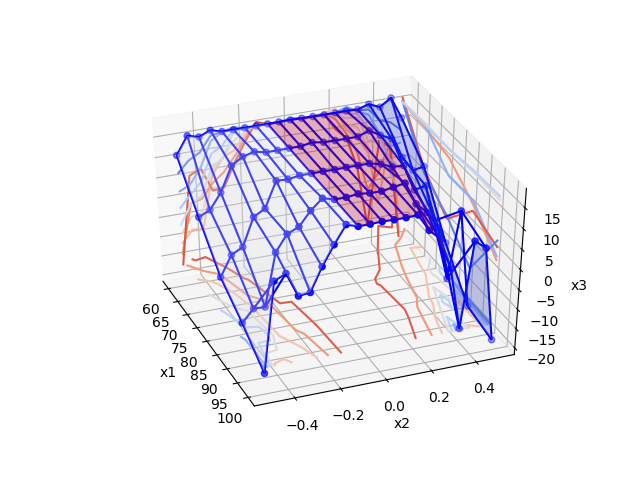
\includegraphics[width=.45\textwidth]{../pics/model_3/X3-x0_0.png}
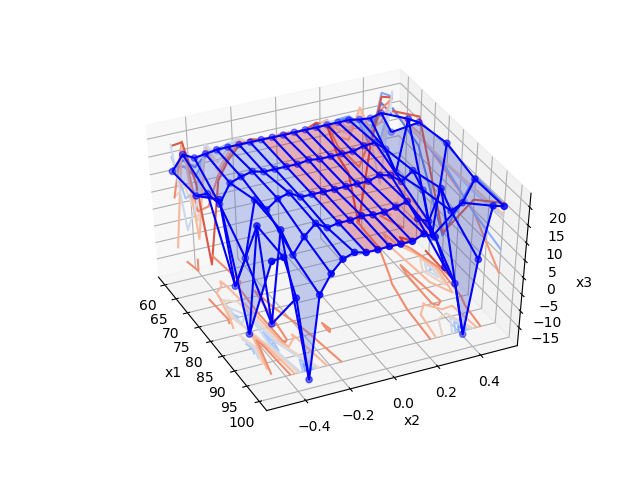
\includegraphics[width=.45\textwidth]{../pics/model_3/X3-x0_1.png}

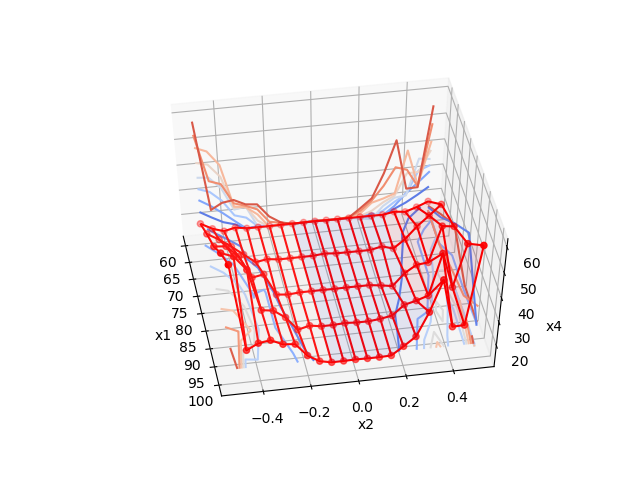
\includegraphics[width=.45\textwidth]{../pics/model_3/X4-x0_0.png}
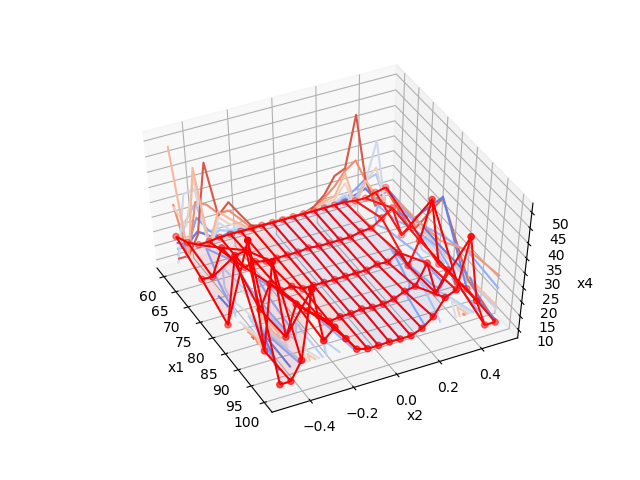
\includegraphics[width=.45\textwidth]{../pics/model_3/X4-x0_1.png}

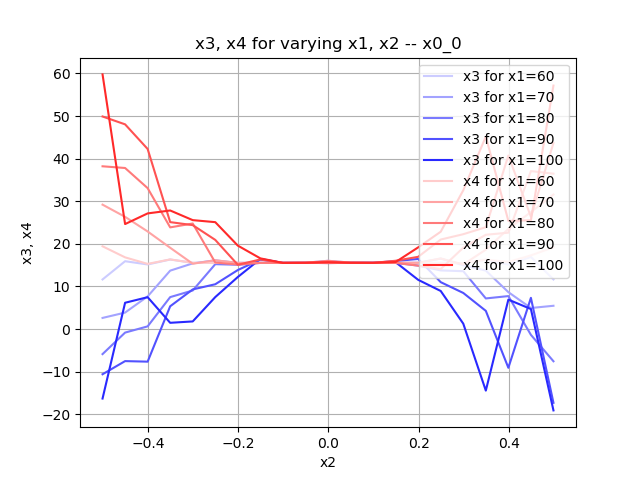
\includegraphics[width=.45\textwidth]{../pics/model_3/X3-X4_-_x0_0_-_2D.png}
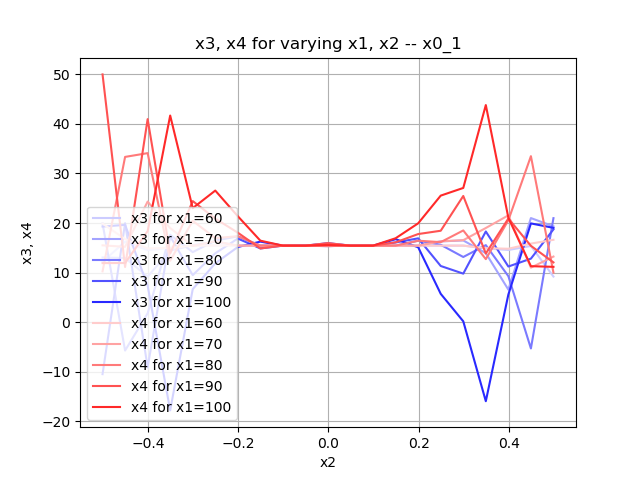
\includegraphics[width=.45\textwidth]{../pics/model_3/X3-X4_-_x0_1_-_2D.png}

\end{document}